\chapter{Experimental Tests in the Solar System}
How can we test relativistic effects in our solar system?
\begin{itemize}
  \item The sum of the mass of all planets is much smaller than the solar mass
  $M_{\astrosun}\approx \unit[2\cdot 10^{30}]{kg}$. The heaviest planet is
  Jupiter with a mass of $M\textsubscript{Jup}\approx \unit[2\cdot
  10^{27}]{kg}$, therefore we can assume the planets to be testparticles.
  \item The sun is in good approximation a spherically symmetric object. We can
  therefore use the Schwarzschild metric.
\end{itemize}
% Consider the variation of the energy functional 
% \begin{equation}
% \int\tensor{g}{_\mu_\nu}\tensor{\dot{x}}{^\mu}\tensor{\dot{x}}{^\nu}\dif\lambda\,.
% \end{equation}
We define
$K:=-\tensor{g}{_\mu_\nu}\tensor{\dot{x}}{^\mu}\tensor{\dot{x}}{^\nu}$, which is
conserved along geodesics and it holds true that
\begin{equation}
K=\begin{cases}
-1& \mathrm{\ timelike\ geodesics}\\
\phantom{-}0& \mathrm{\ lightlike\ geodesics}
\end{cases}\,.
\end{equation}
Using the Schwarzschild metric, we can explicitly write
\begin{equation}
K=-e^{2a(r)}\dot{t}^2+e^{2b(r)}\dot{r}^2+r^2\left(\dot{\vartheta}+\sin^2\vartheta
\dot{\phi}\right)
\end{equation}
A Killing-vector $\tensor{\xi}{^\mu}$ satisfies
\begin{equation}
\tensor{\xi}{_\mu}\tensor{\dot{x}}{^\mu}=\mathrm{\ const.}
\end{equation}
For the Schwarzschild metric, there are four independent Killing-vectors,
corresponding to 3 rotations, and staticity (time independence).
Conservation of angular momentum leads to a motion in a plane, w.l.o.g.\ we can
chose a coordinate system in which $\vartheta=\nicefrac{\pi}{2}$.
The Killing-Vectors are given by
\begin{align}
\tensor*{\xi}{_{(\varphi)}^\mu}&=(\partial_\varphi)^\mu=\tensor*{\delta}{_\varphi^\mu}\,,\\
\tensor*{\xi}{_{(t)}^\mu}&=(\partial_t)^\mu=\tensor*{\delta}{_t^\mu}\,.
\end{align}
The associated conserved quantities are
\begin{align}
E&:=\tensor*{\xi}{_{(\varphi)}^\mu}\tensor{g}{_\mu_\nu}\tensor{\dot{x}}{^\nu}
=\tensor{g}{_t_t}\dot{t}
=e^{2a}\dot{t}
=\left(1-\frac{2M}{r}\right)\dot{t}
\\
L&:=\tensor*{\xi}{_{(t)}^\mu}\tensor{g}{_\mu_\nu}\tensor{\dot{x}}{^\nu}
=\tensor{g}{_\varphi_\varphi}\dot{\varphi}
=r^2\dot{\varphi}\,.
\end{align}
For massless
%TODO stimmt das?
particles, we can think of $E$ and $L$ as conserved energy and angular momentum.
It follows
\begin{equation}
K=-\left(1-\frac{2M}{r}\right)\dot{t}^2+\left(1-\frac{2M}{r}\right)^{-1}\dot{r}^2+r^2\varphi^2
\end{equation}
If we insert the conserved quantities $L,E$ and multiply by
$\frac{1}{2}\left(1-\frac{2M}{r}\right)$, we get
\begin{equation}
\frac{E^2}{2}=\frac{\dot{r}^2}{2}
+\left(1-\frac{2M}{r}\right)\left(\frac{L^2}{2r}-\frac{K}{2}\right)\,.
\end{equation}
This expression can be rearranged to the Form
\begin{equation}
\frac{\dot{r}^2}{2}+V\textsubscript{eff}(r)
=\varepsilon\,,
\end{equation}
with the convenient definitions 
\begin{equation}
V\textsubscript{eff}(r):=\frac{MK}{r}+\frac{L^2}{2r^2}-\frac{ML^2}{r^3}\,,\quad
\varepsilon:=\frac{E^2+K}{2}\,.
\end{equation}
\section{Perihelion Shift of Mercury}
\begin{figure}[b]
\centering
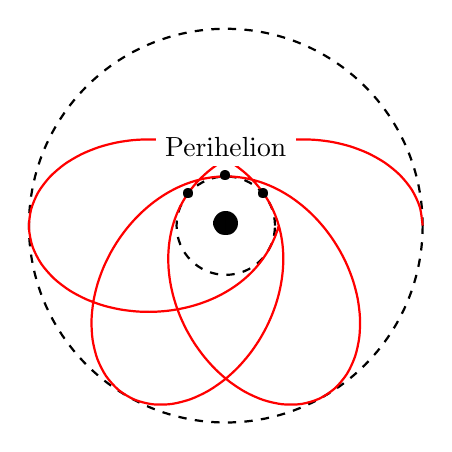
\begin{tikzpicture}[auto,node distance=3cm,thick,main node/.style={circle,draw,font=\sffamily\Large\bfseries}]
\draw [black,thick,dashed] (0,0) circle (1/1.6);
\draw [black,thick,dashed] (0,0) circle (1/0.4);
\draw [thick, color=red, domain=0:6*pi, samples=200, smooth]
  plot (xy polar cs:angle=\x r, radius={1/(1-0.6*cos(\x r+0.2*\x r))});
\node [fill=white] at (0,1) {Perihelion};s
\node at (0,0) {\Huge\textbullet};
\node (1) at (40:1/1.6) {\textbullet};
\node (2) at (90:1/1.6) {\textbullet};
\node (3) at (140:1/1.6) {\textbullet};
\end{tikzpicture} 
\caption{Perhelion shift of mercury (exaggerated)}
\end{figure}
It has been known for a long time that the perihelion of the mercury moves by
roughly $5061''\footnote{Where an arcsec $''$ denotes the 3600 part of
an degree.}/\textrm{century}$, if on subtracts other effects such a
fraction of $43''/\textrm{century}$. 
There where several proposed explanations for this including
\begin{itemize}
  \item a new planet called Vulcan between mercury and the sun,
  \item a change to newtons $1/r^2$-law,
  \item effects due the suns quadrupole moment. 
\end{itemize}
We will now look at what is predicted by GR.
The trajectories of planets ($K=-1$) are given by
\begin{equation}
\dot{r}^2-\frac{2M}{r}+\frac{L^2}{r^2}-\frac{2ML^2}{r^3}=E^2-1\label{eq:planeteq}\,.
\end{equation}
If we think of the radius as a function of the angle, we can write
\begin{equation}
\dot{r}=\od{r}{\lambda}=\od{r}{\phi}\od{\phi}{\lambda}\,.
\end{equation}
Multiplying \eqref{eq:planeteq} with
%TODO choose between varphi and phi
$\left(\od{\phi}{\lambda}\right)^{-2}=\frac{1}{\dot{\phi}}=\frac{r^4}{L^2}$
yields
\begin{equation}
\left(\dod{r}{\phi}\right)^2-\frac{2Mr^3}{L^2}+r^2-2Mr
=\left(E^2-1\right)\frac{r^4}{L^2}\,.\label{eq:orbitrphi}
\end{equation}
Similar to the treatment of the Keppler problem in classical mechanics, we
define
\begin{equation}
u(\phi):=\frac{L^2}{Mr(\phi)}\,.
\end{equation}
This implies
\begin{equation}
\dif r=-\frac{L^2}{Mu^2}\dif u\,,\quad
\left(\dod{r}{\phi}\right)^2=\frac{L^4}{M^2u^4}\left(\dod{u}{\phi}\right)^2\,.
\end{equation}
In terms of the new variables \eqref{eq:orbitrphi} reads
\begin{equation}
\left(\dod{u}{\phi}\right)^2-2u+u^2-\frac{2M^2}{L^2}u^3=(E^2-1)\frac{L^2}{M^2}\,.
\end{equation}
We differentiate with respect to $\phi$ and get 
\footnote{primes denote $\phi$
derivatives}
\begin{equation}
2u^\prime u^{\prime\prime}-2u^\prime+2u
u^{\prime}-\frac{6M^2}{L^2}u^2u^\prime=0\,.
\end{equation}
Dividing by $2u^\prime$ yields
\begin{equation}
u^{\prime\prime}-1+u=\frac{3M^2}{L^2}u^2\,,
\end{equation}
which is an equation similar to the Keppler problem. The difference is in the
right hand side, which is equal zero in the classical case.
We may calculate an approximation by pertubative corrections
\footnote{The quantity relevant for the error of a given order is
$\frac{3M^2}{L^2}$.}
\begin{equation}
u=u_0+u_1+u_2+\dots\,.
\end{equation}
At zeroth order, we neglect the quadratic term, so that we are left with
\begin{equation}
u_0^{\prime\prime}-1+u_0=0\,,
\end{equation}
which is equal to the Newtonian problem, with exact solution
\begin{equation}
u_0(\phi)=1+\varepsilon\cos\phi\,.
\end{equation}
At first order we have
\begin{equation}
\begin{split}
u_1^{\prime\prime}-1+u_1&=\frac{3M^2}{L^2}u_0^2\\
&=\frac{3M^2}{L^2}\left(1+\varepsilon\cos\phi\right)^2\\\
&=\frac{3M^2}{L^2}\left(1+\frac{\varepsilon^2}{2}+2\varepsilon\cos\phi+\frac{1}{2}\varepsilon^2\cos
2\phi\right)\,,
\end{split}
\end{equation}
Where we made use of trigonometric identities in the last step. 
The first order solution reads
\begin{equation}
u_1(\phi)=1+\varepsilon\cos\phi+\frac{3M^2}{L^2}\phi\sin\phi\,.
\end{equation}
which can be checked by using
\begin{align}
\dod[2]{}{\phi}(\phi\sin\phi)+\phi\sin\phi&=2\cos\phi\,,\\
\dod[2]{}{\phi}(\cos 2\phi)+\cos 2\phi&=-3\cos 2\phi\,.
\end{align}
Assuming that we still have approximately a movement along an ellipse and Taylor
expansion yields
\begin{equation}
u(\phi)=1+\varepsilon\cos[(1-\delta)\phi]
\simeq
1+\varepsilon\cos\phi
+\varepsilon\delta\phi\sin\phi+\landauO(\delta^2)\,.
\end{equation}
Comparing this to the expression for $u_1$ we find
\begin{equation}
\delta=\frac{3M^2}{L^2}
\end{equation}
and the error is of order $\delta^2$.
%\begin{equation}
% r(\phi)=\frac{p}{1+\varepsilon\cos\phi}
% =\frac{a\left(1-\varepsilon^2\right)}{1+\varepsilon\cos\phi}
% \end{equation}
If we assume that there was a perihelion at $\phi_p$, the next one will occure
at $\phi+\Delta\Phi$ with 
\begin{equation}
\Delta\phi=2\pi\delta=\frac{6\pi M^2}{L^2}
\end{equation}
The zeroth order solution gives 
\begin{equation}
r_0(\phi)=\frac{L^2}{M(1+\varepsilon\cos\phi)}\stackrel{!}{=}
\frac{a(1-\varepsilon^2)}{1+\varepsilon\cos\phi}\,.
\end{equation}
So $L^2\approx M(1-\varepsilon^2)a$ with an error of order $\delta$, that can
be neglected.
With this approximation and restoring factors of $c$ and $G$ we arrive at the following
expression for the perihelion shift:
\begin{equation}
\Delta\phi=\frac{6\pi G M_{\astrosun}}{c^2 (1-\varepsilon^2)a}\,.
\end{equation}
As expected the effect scalses with $1/a$ and thus the planet nearest to the sun
recives the strongest effect. For mercury we have
\begin{equation}
\frac{GM_{\astrosun}}{c^2}=\unit[1.48]{km}\,,\quad a =\unit[5.79\cdot
10^7]{km}\,,\quad\varepsilon=0.2056\,,
\end{equation}
Which results in an perihelionshift
\begin{equation}
\Delta\phi\textsubscript{mer}
=\unitfrac[5.03\cdot 10^{-7}]{rad}{orbit}
=\unitfrac[43]{{}^{\prime\prime}}{century}\,,
\end{equation}
which fits the observation in the error margin.